
	En el punto anterior se describió el algoritmo de Kalman. En el mismo hay una fase de inicialización de la estimación. En esta Sección se analizan las variaciones que se presentan a la hora de cambiar los valores iniciales. Por ejemplo se podría inicializar en un valor coincidente con los datos, con una varianza pequeña, en cuyo caso la estimación convergerá más rápido. Otro caso extremo es cuando el valor inicial es incorrecto, también con varianza pequeña, resultando en una convergencia mucho más lenta. La idea de este punto es la exploración de las distintas variantes de este tema y en cada caso se presentarán gráficos de la estimación de la trayectoria, de evolución de los errores y de la autocorrelación de las innovaciones.
	
	\subsection{Caso 1 - $\vect{x}_{0/0} = [40\;-200\;0\;0\;0\;0]^T$, $P^{'}_{0/0}=100\; P_{0|0}$} \label{sec:ej3a}
	
		Para el primer caso, se tiene un error en la estimación del estado inicial pequeño, pero una varianza grande. En este caso el algoritmo convergerá rápidamente a la trayectoria real. El resultado puede verse en la Figura \ref{fig:ej3a}.
	
		\begin{figure}[H]
			\centering
			%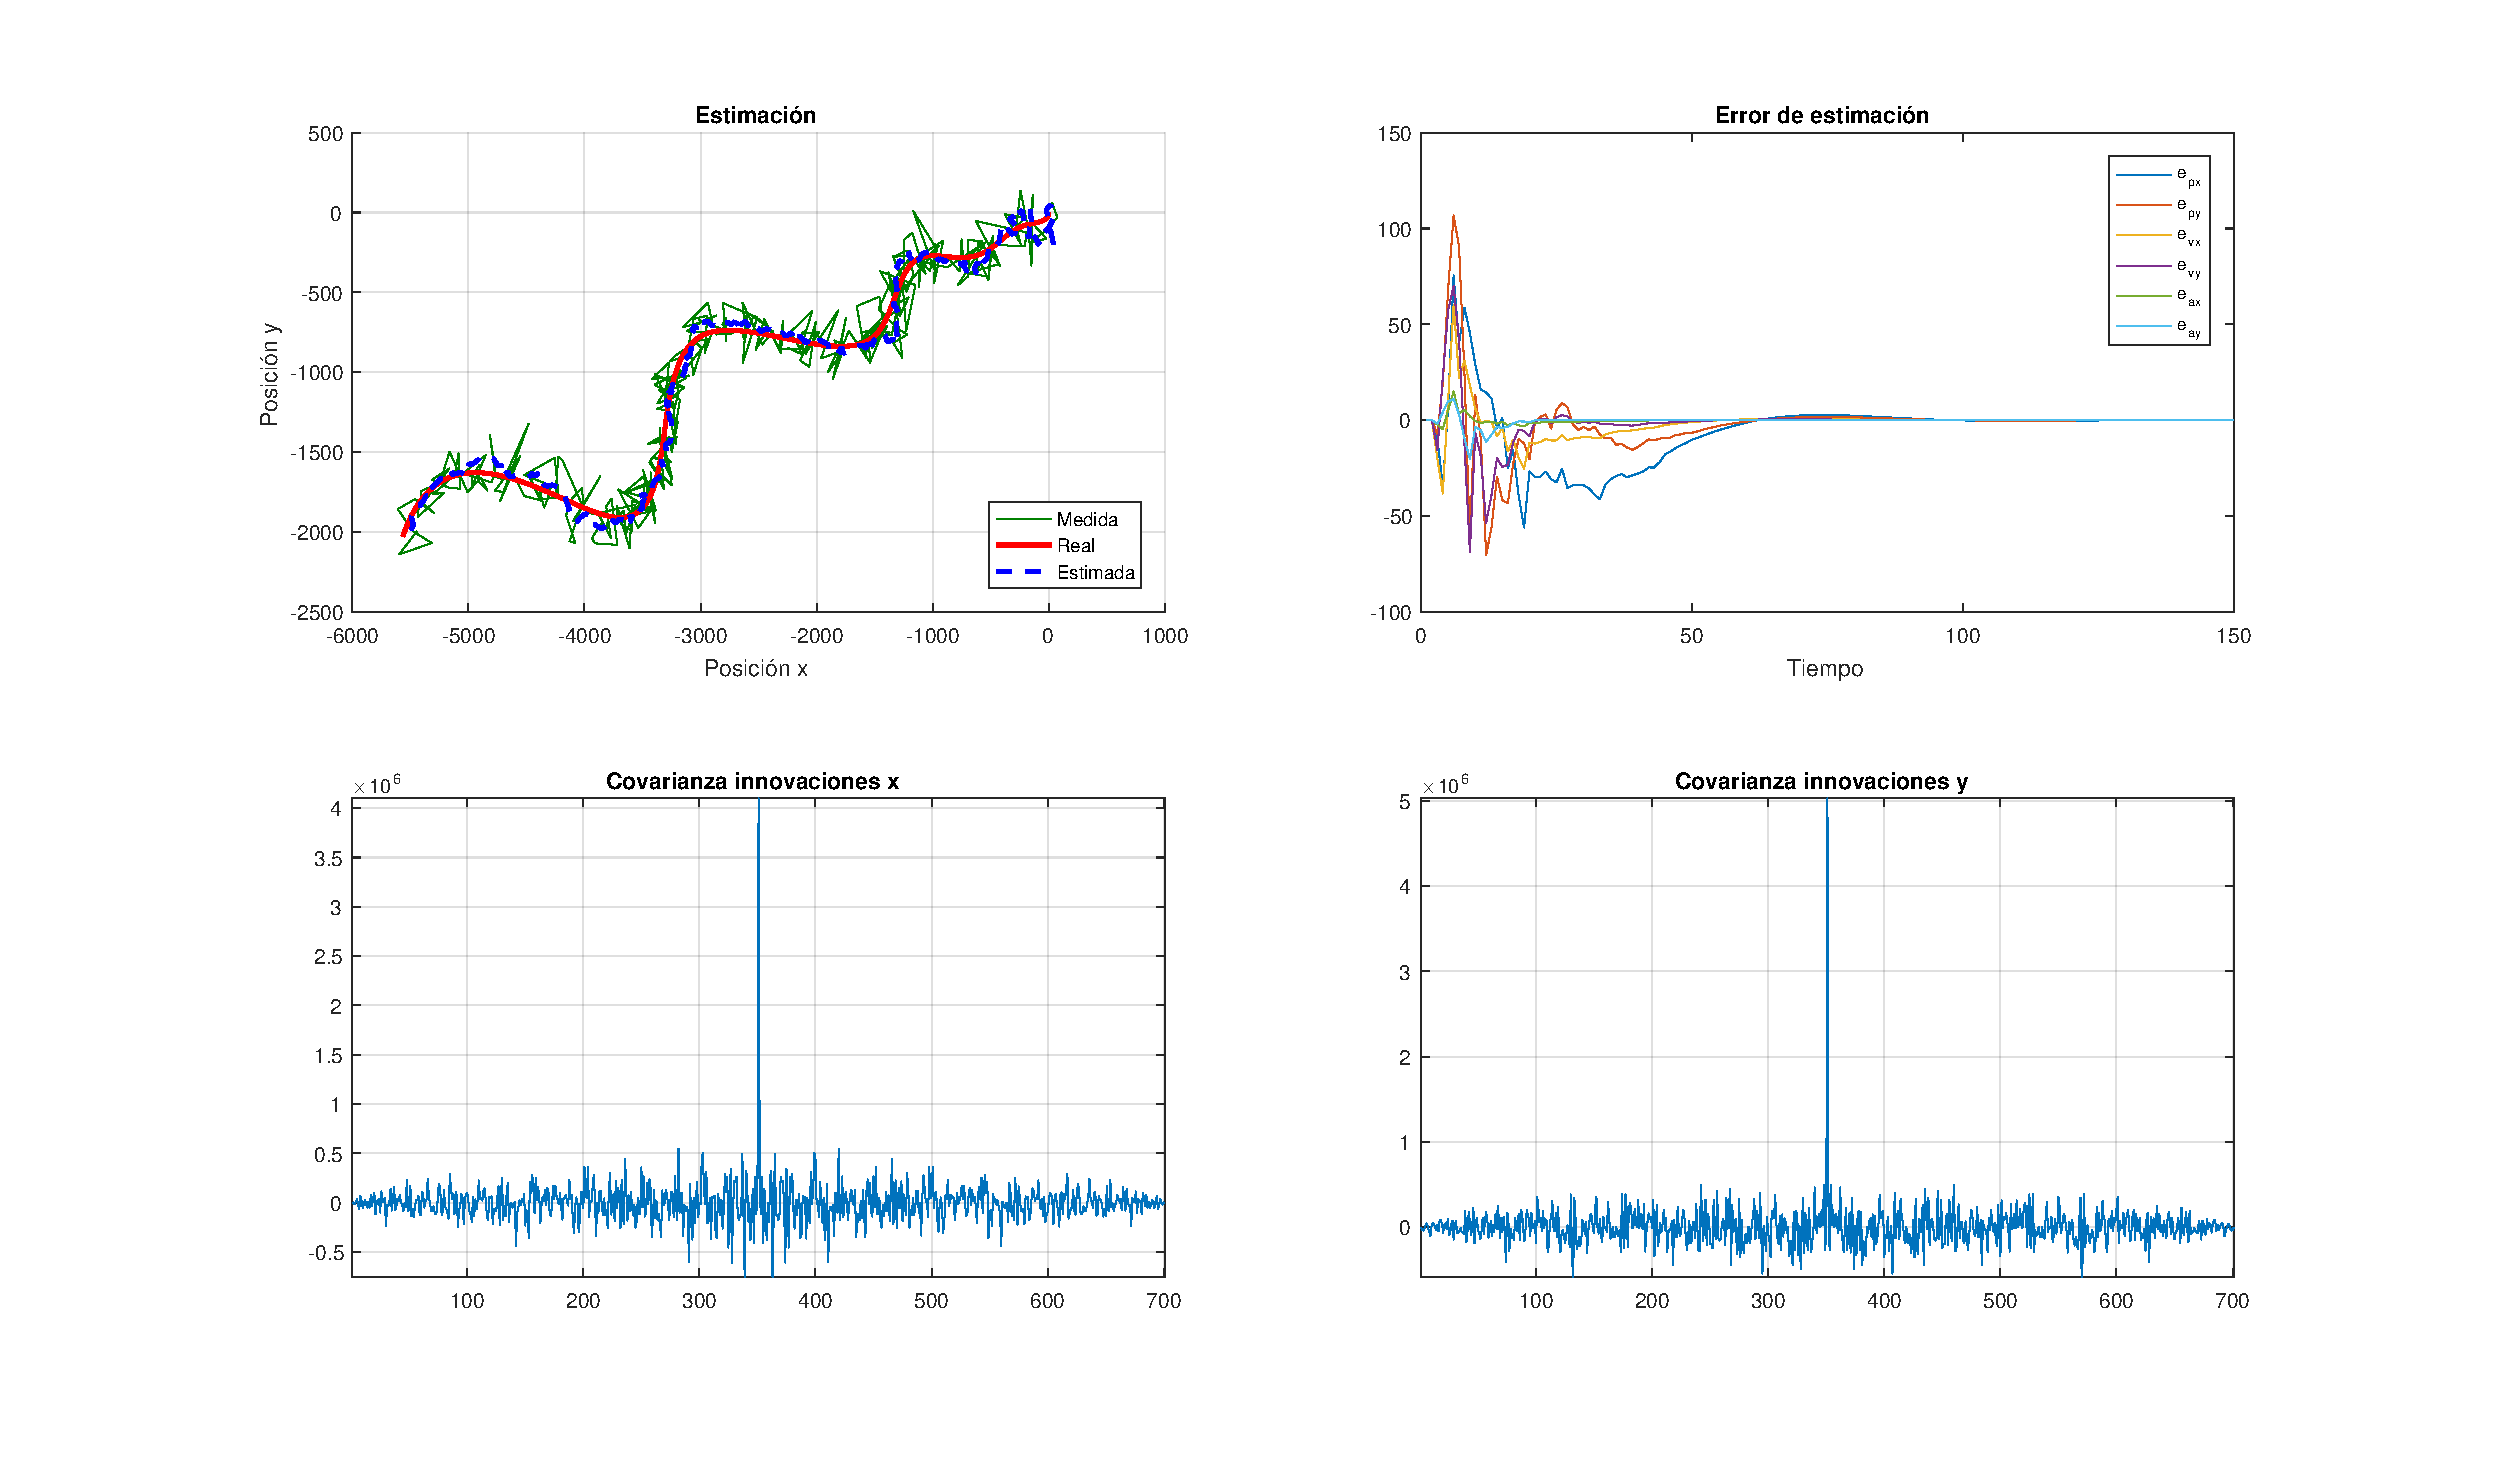
\includegraphics[width=1.0\textwidth,keepaspectratio]{Figuras/graf_ej3a.pdf}
			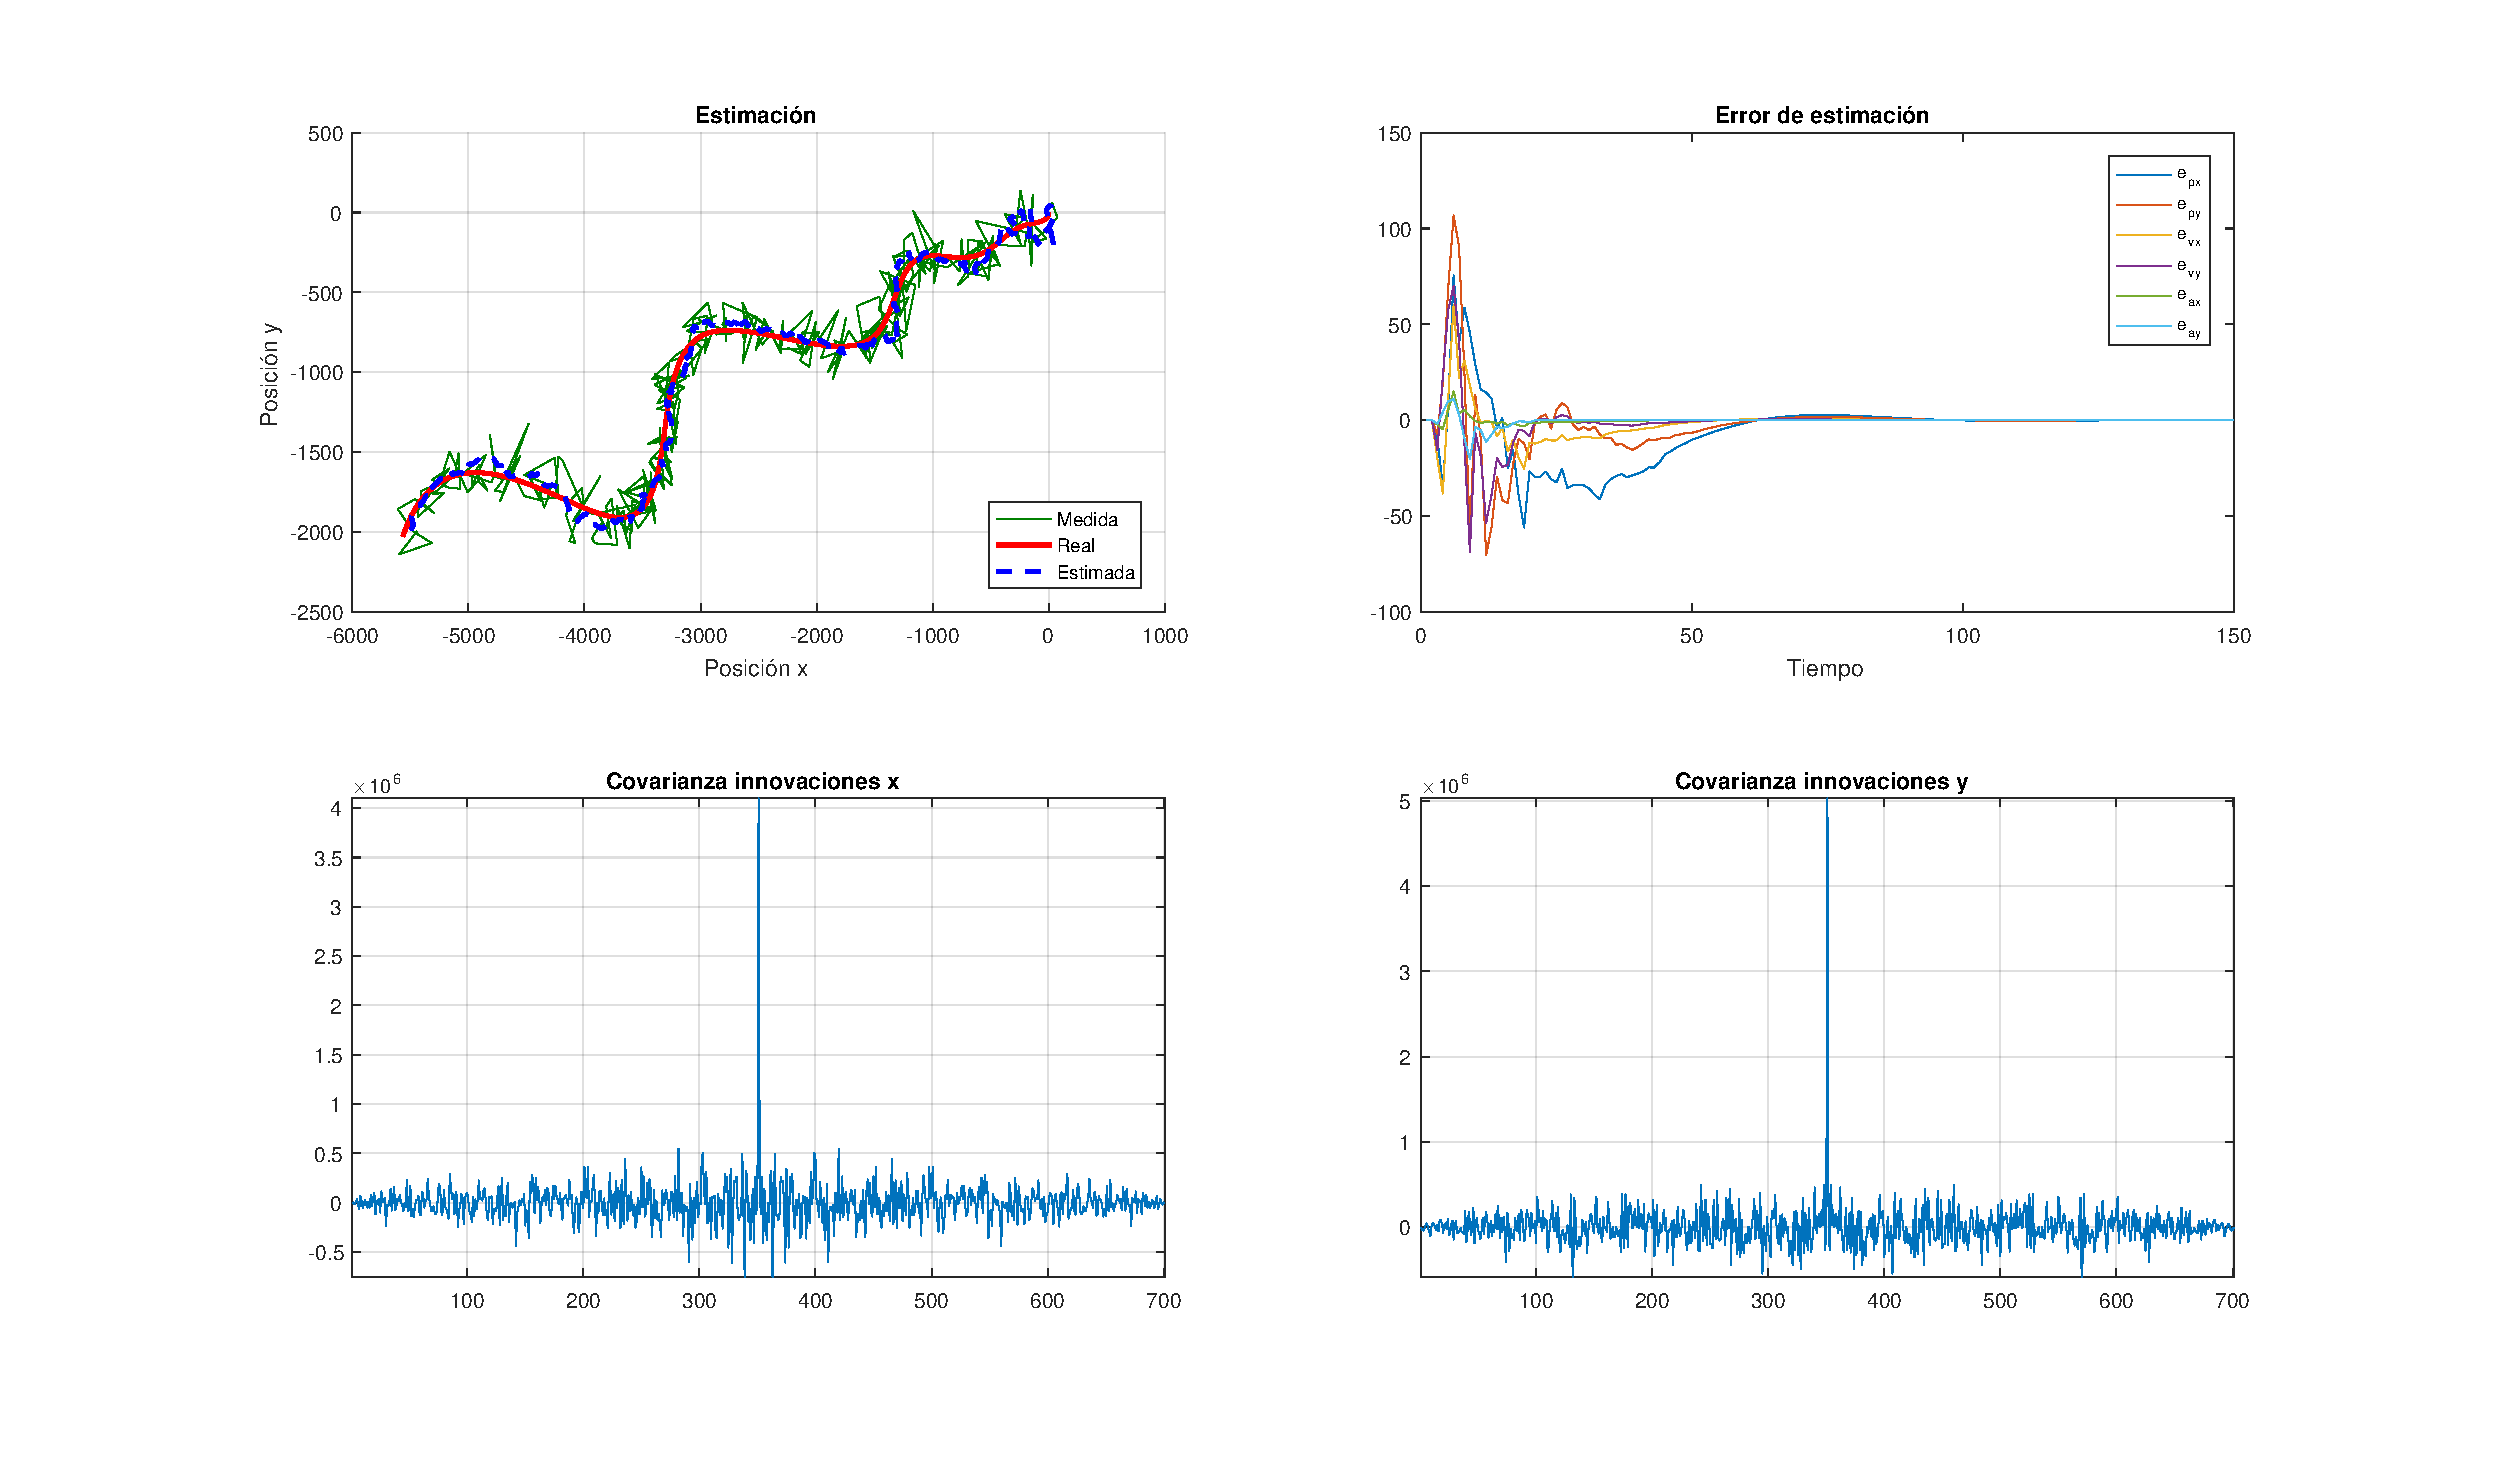
\includegraphics[scale=0.5,trim={6,5cm 0 0 0}]{Figuras/graf_ej3a.pdf}
			\caption{Caso 1}
			\label{fig:ej3a}
		\end{figure}
	
	\subsection{Caso 2 - $\vect{x}_{0/0} = [200\;-3000\;0\;0\;0\;0]^T$, $P^{'}_{0/0}=100\; P_{0|0}$} \label{sec:ej3b}
	
	Ahora se tiene un error en el estado inicial grande, pero al ser la varianza grande el algoritmo sabe que se trata de un valor poco confiable, y no tarda demasiado en corregir la estimación de la trayectoria. El resultado puede verse en la Figura \ref{fig:ej3b}.
		
		\begin{figure}[H]
			\centering
			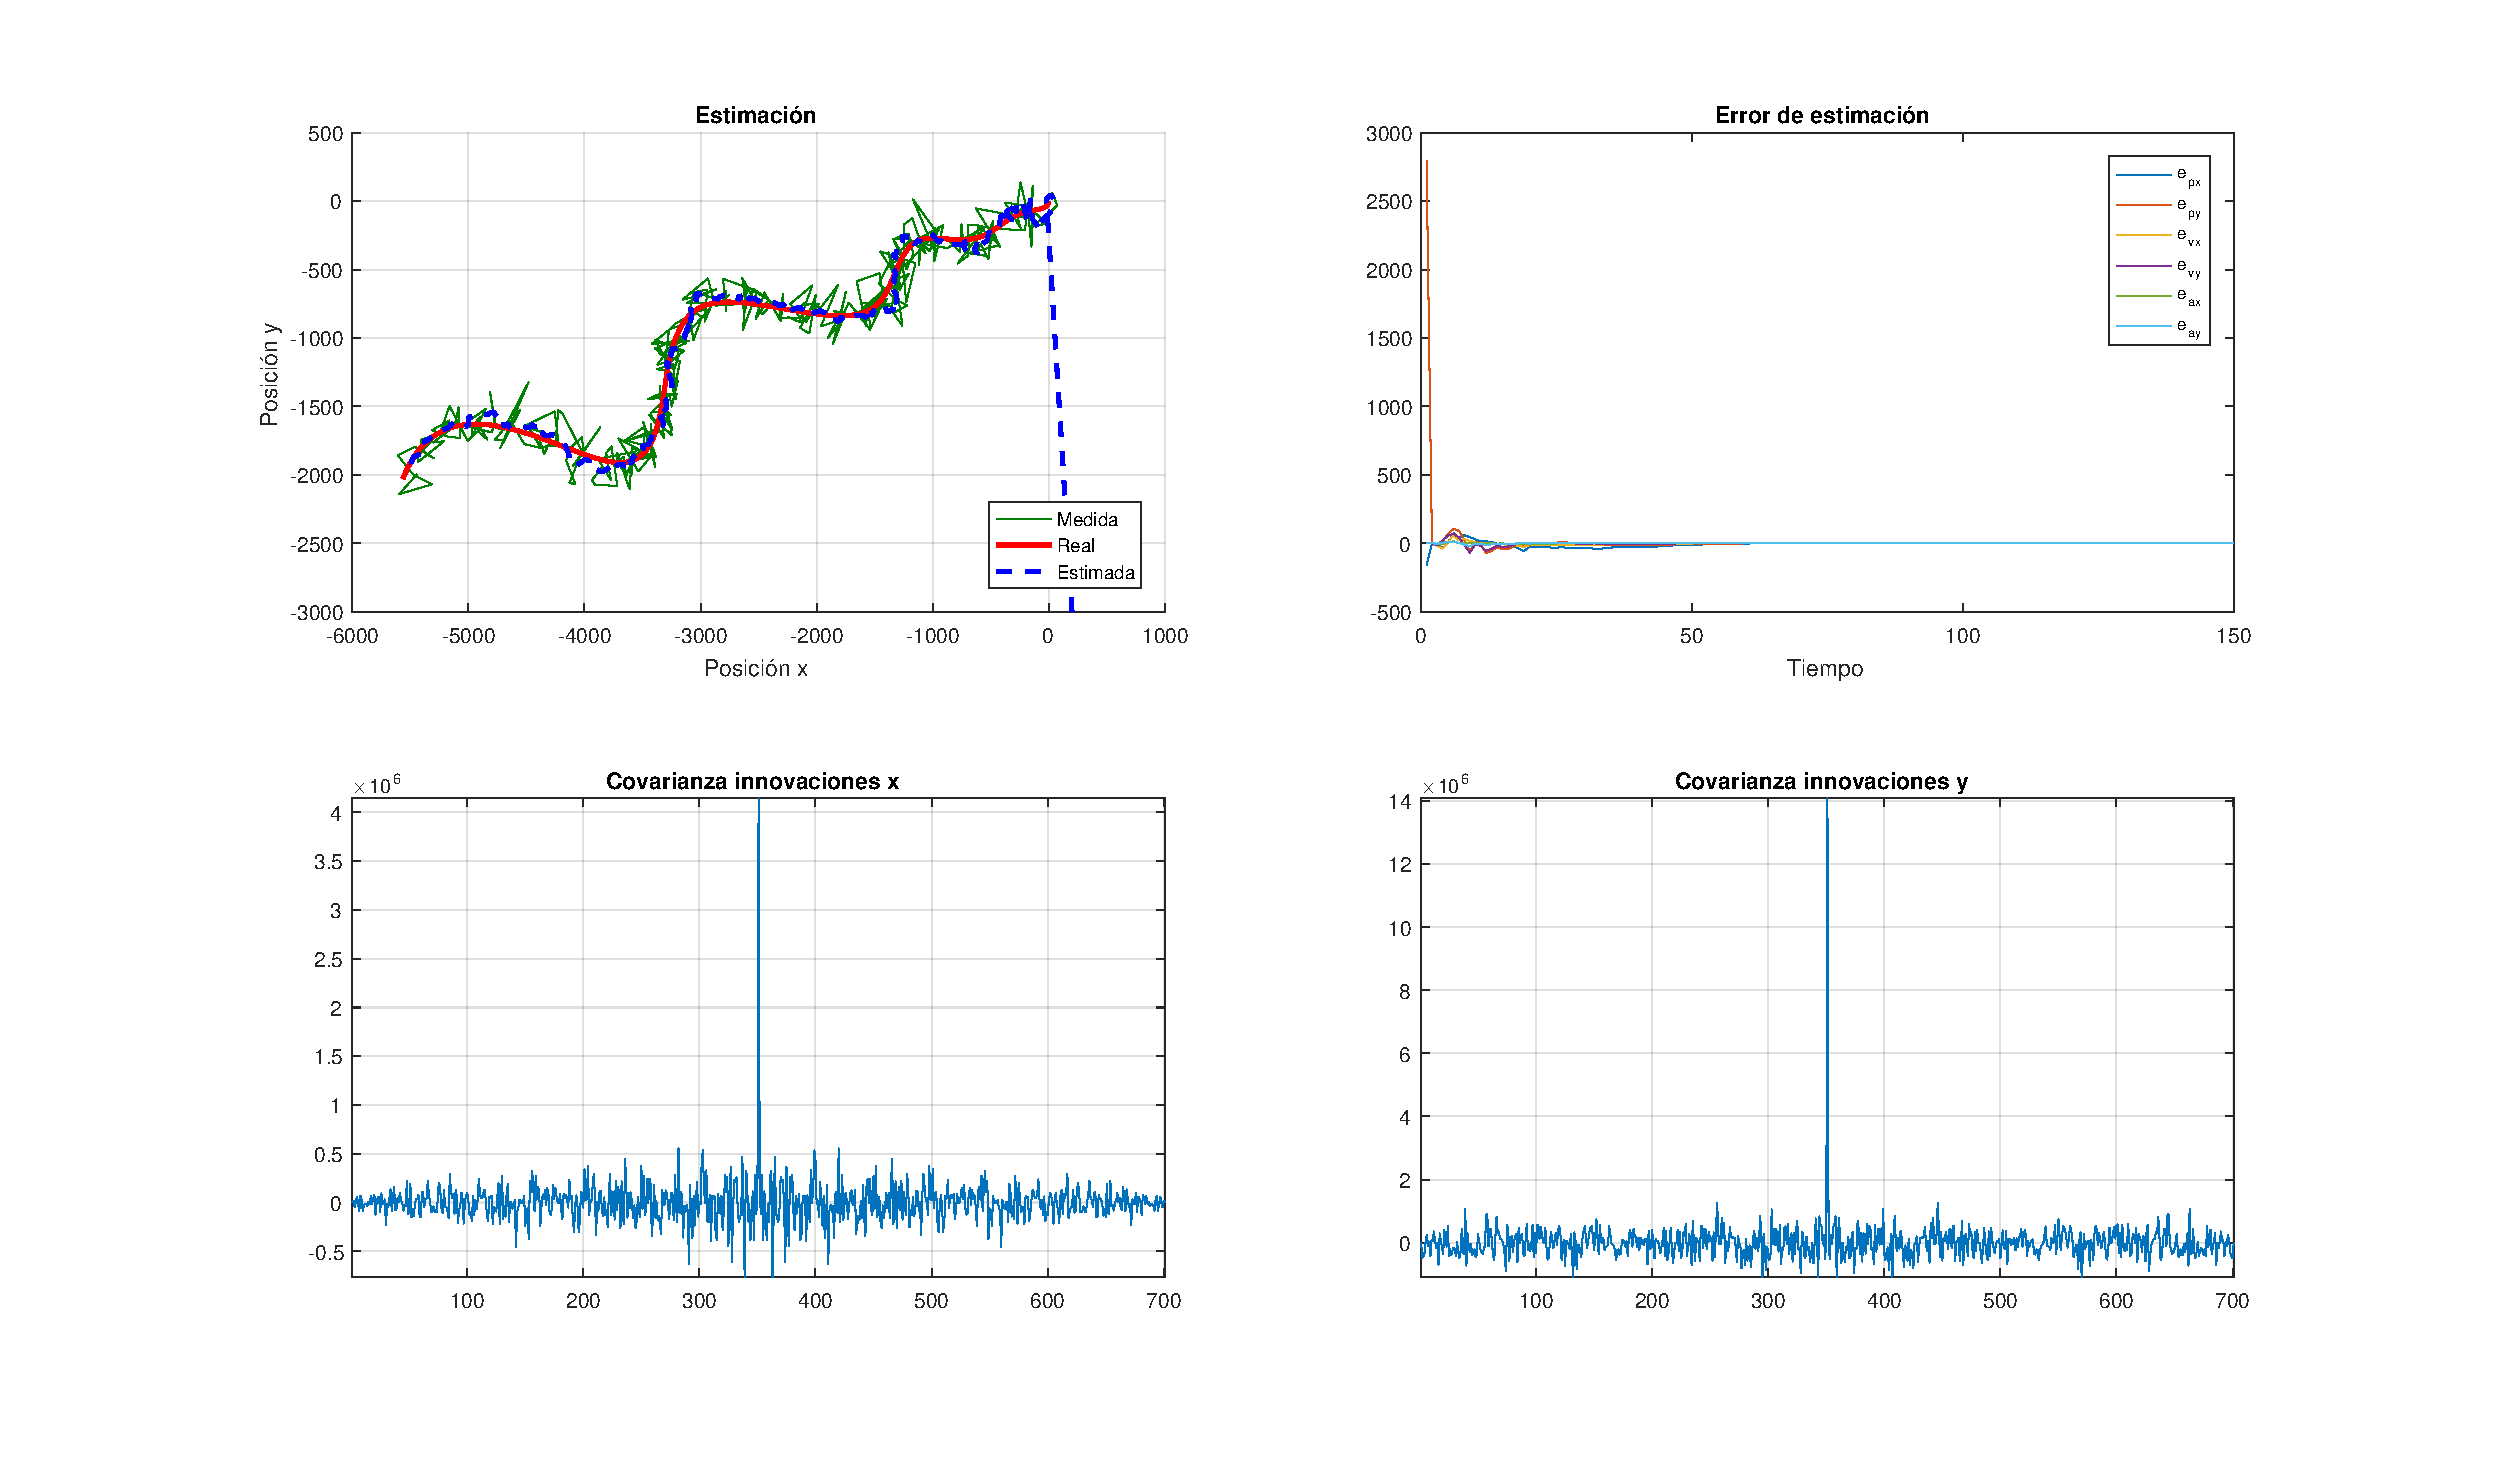
\includegraphics[scale=0.5,trim={6,5cm 0 0 0}]{Figuras/graf_ej3b.pdf}
			\caption{Caso 2}
			\label{fig:ej3b}
		\end{figure}
	\indent Se observa que a comparación a \ref{sec:ej3a}, teniendo una covarianza grande en ambos, el algorítmo converge más rápido con posición inicial más distante del valor real. Al tener un valor inicial más cercano al verdadero, la correlación de las mediciones con dicho valor es menor implicando en innovaciones con menor varianza. Como $P$ es grande, el algoritmo de Kalman genera una ganancia $K$ grande causando que los valores de $\vect{x}_{k/k}$ sigan más a la innovación (medición) que a la predicción a través de la dinámica. En consecuencia, con $P$ grande el algoritmo converge más rápido si el valor inicial no se asemeja al valor verdadero para que las innovaciones provean más información.
	
	\subsection{Caso 3 - $\vect{x}_{0/0} = [40\;-200\;0\;0\;0\;0]^T$, $P^{'}_{0/0}=\num{0.01}\; P_{0|0}$} \label{sec:ej3c}
	
	En este tercer caso el error de la estimacion del estado inicial es pequeño, pero a diferencia del primer caso la varianza es grande. Dado ésto, el algoritmo se confia menos del valor inicial y tarda más en converger que en el primer caso (convergencia del error en \SI{100}{\s} versus \SI{60}{\s}). El resultado puede verse en la Figura \ref{fig:ej3c}.
	
		\begin{figure}[H]
			\centering
			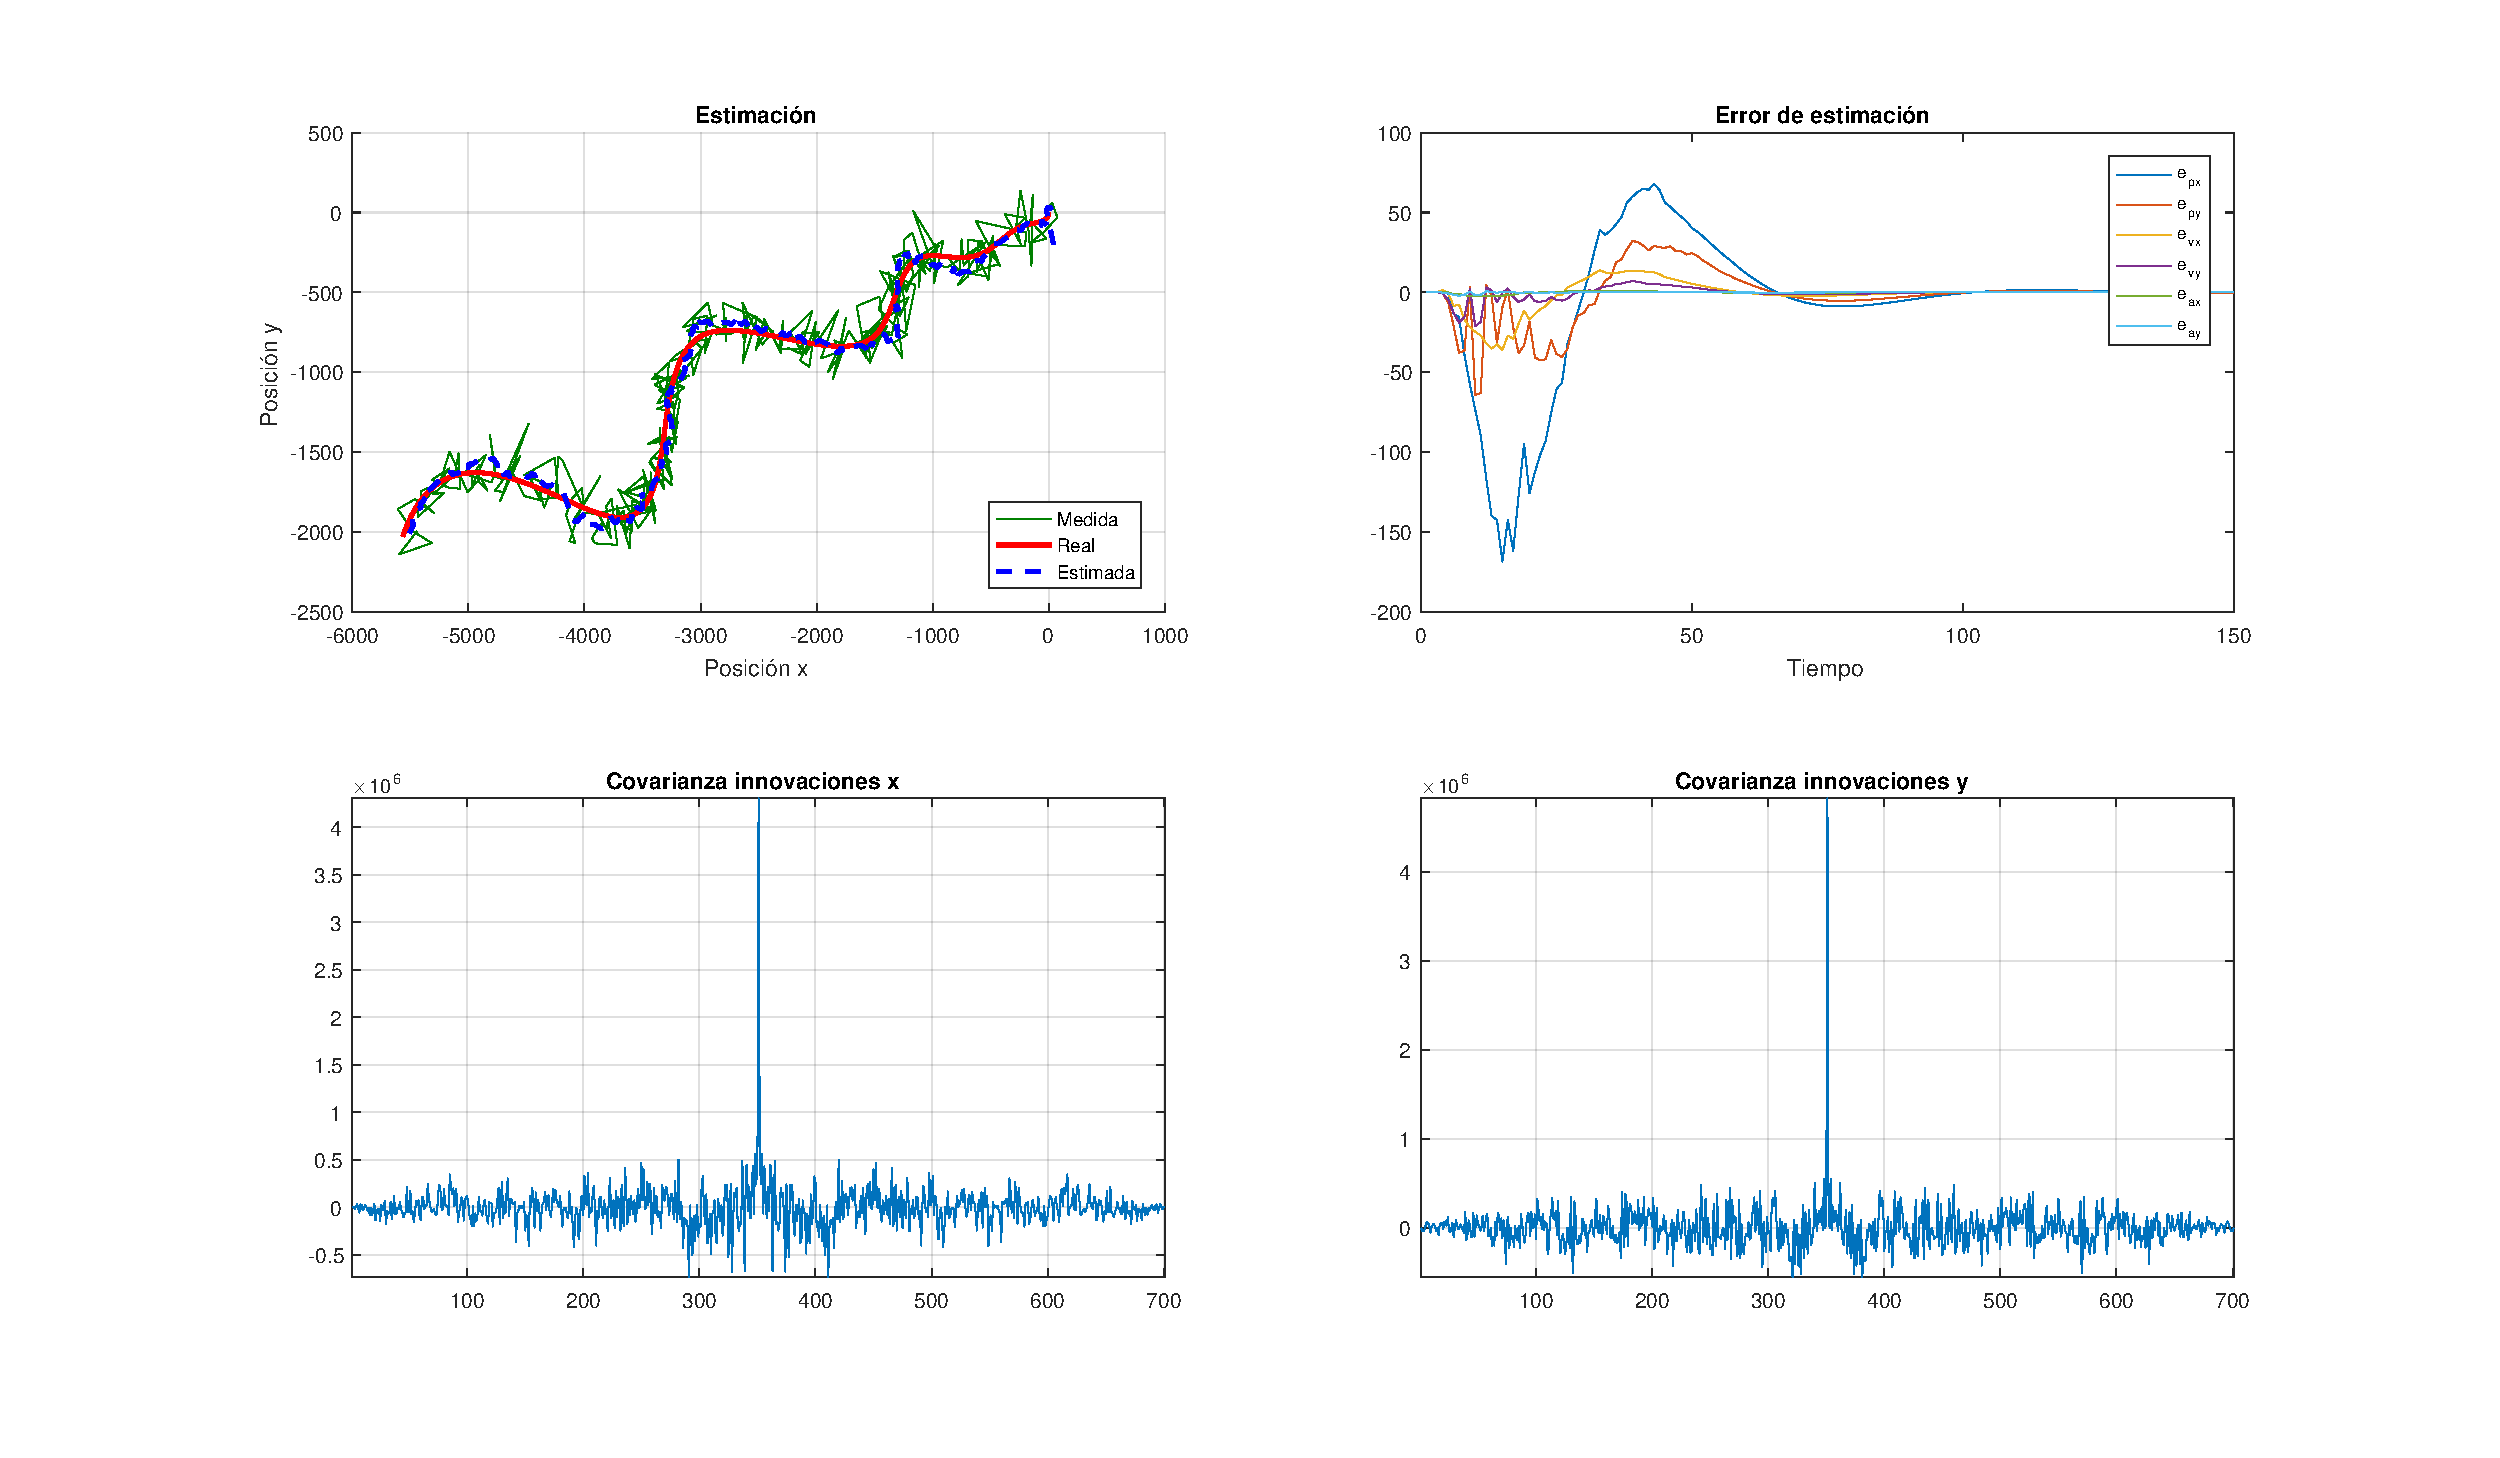
\includegraphics[scale=0.5,trim={6,5cm 0 0 0}]{Figuras/graf_ej3c.pdf}
			\caption{Caso 3}
			\label{fig:ej3c}
		\end{figure}
	
	\subsection{Caso 4 - $\vect{x}_{0/0} = [200\;-30000\;0\;0\;0\;0]^T$, $P^{'}_{0/0}=\num{0.01}\; P_{0|0}$} \label{sec:ej3d}
	
	Finalmente cuando se trata de un error en el estado inicial grande con una varianza pequeña, se ve que es el peor caso. Se está inicializando el algoritmo con un estado incorrecto y además se le está informando que es muy confiable. En el algoritmo en sí se puede ver que con $P$ bajo, se desprecia el aporte de las innovaciones siguiendo la dinámica a partir del valor inicial. Sin embargo, al distar mucho del verdadero, la trayectoria estimada tarda mucho en estabilizarse con respecto a la real (se ve que sigue oscilando para tiempos mayores a \SI{100}{\s}). El resultado puede verse en la Figura \ref{fig:ej3d}.
	
		\begin{figure}[H]
			\centering
			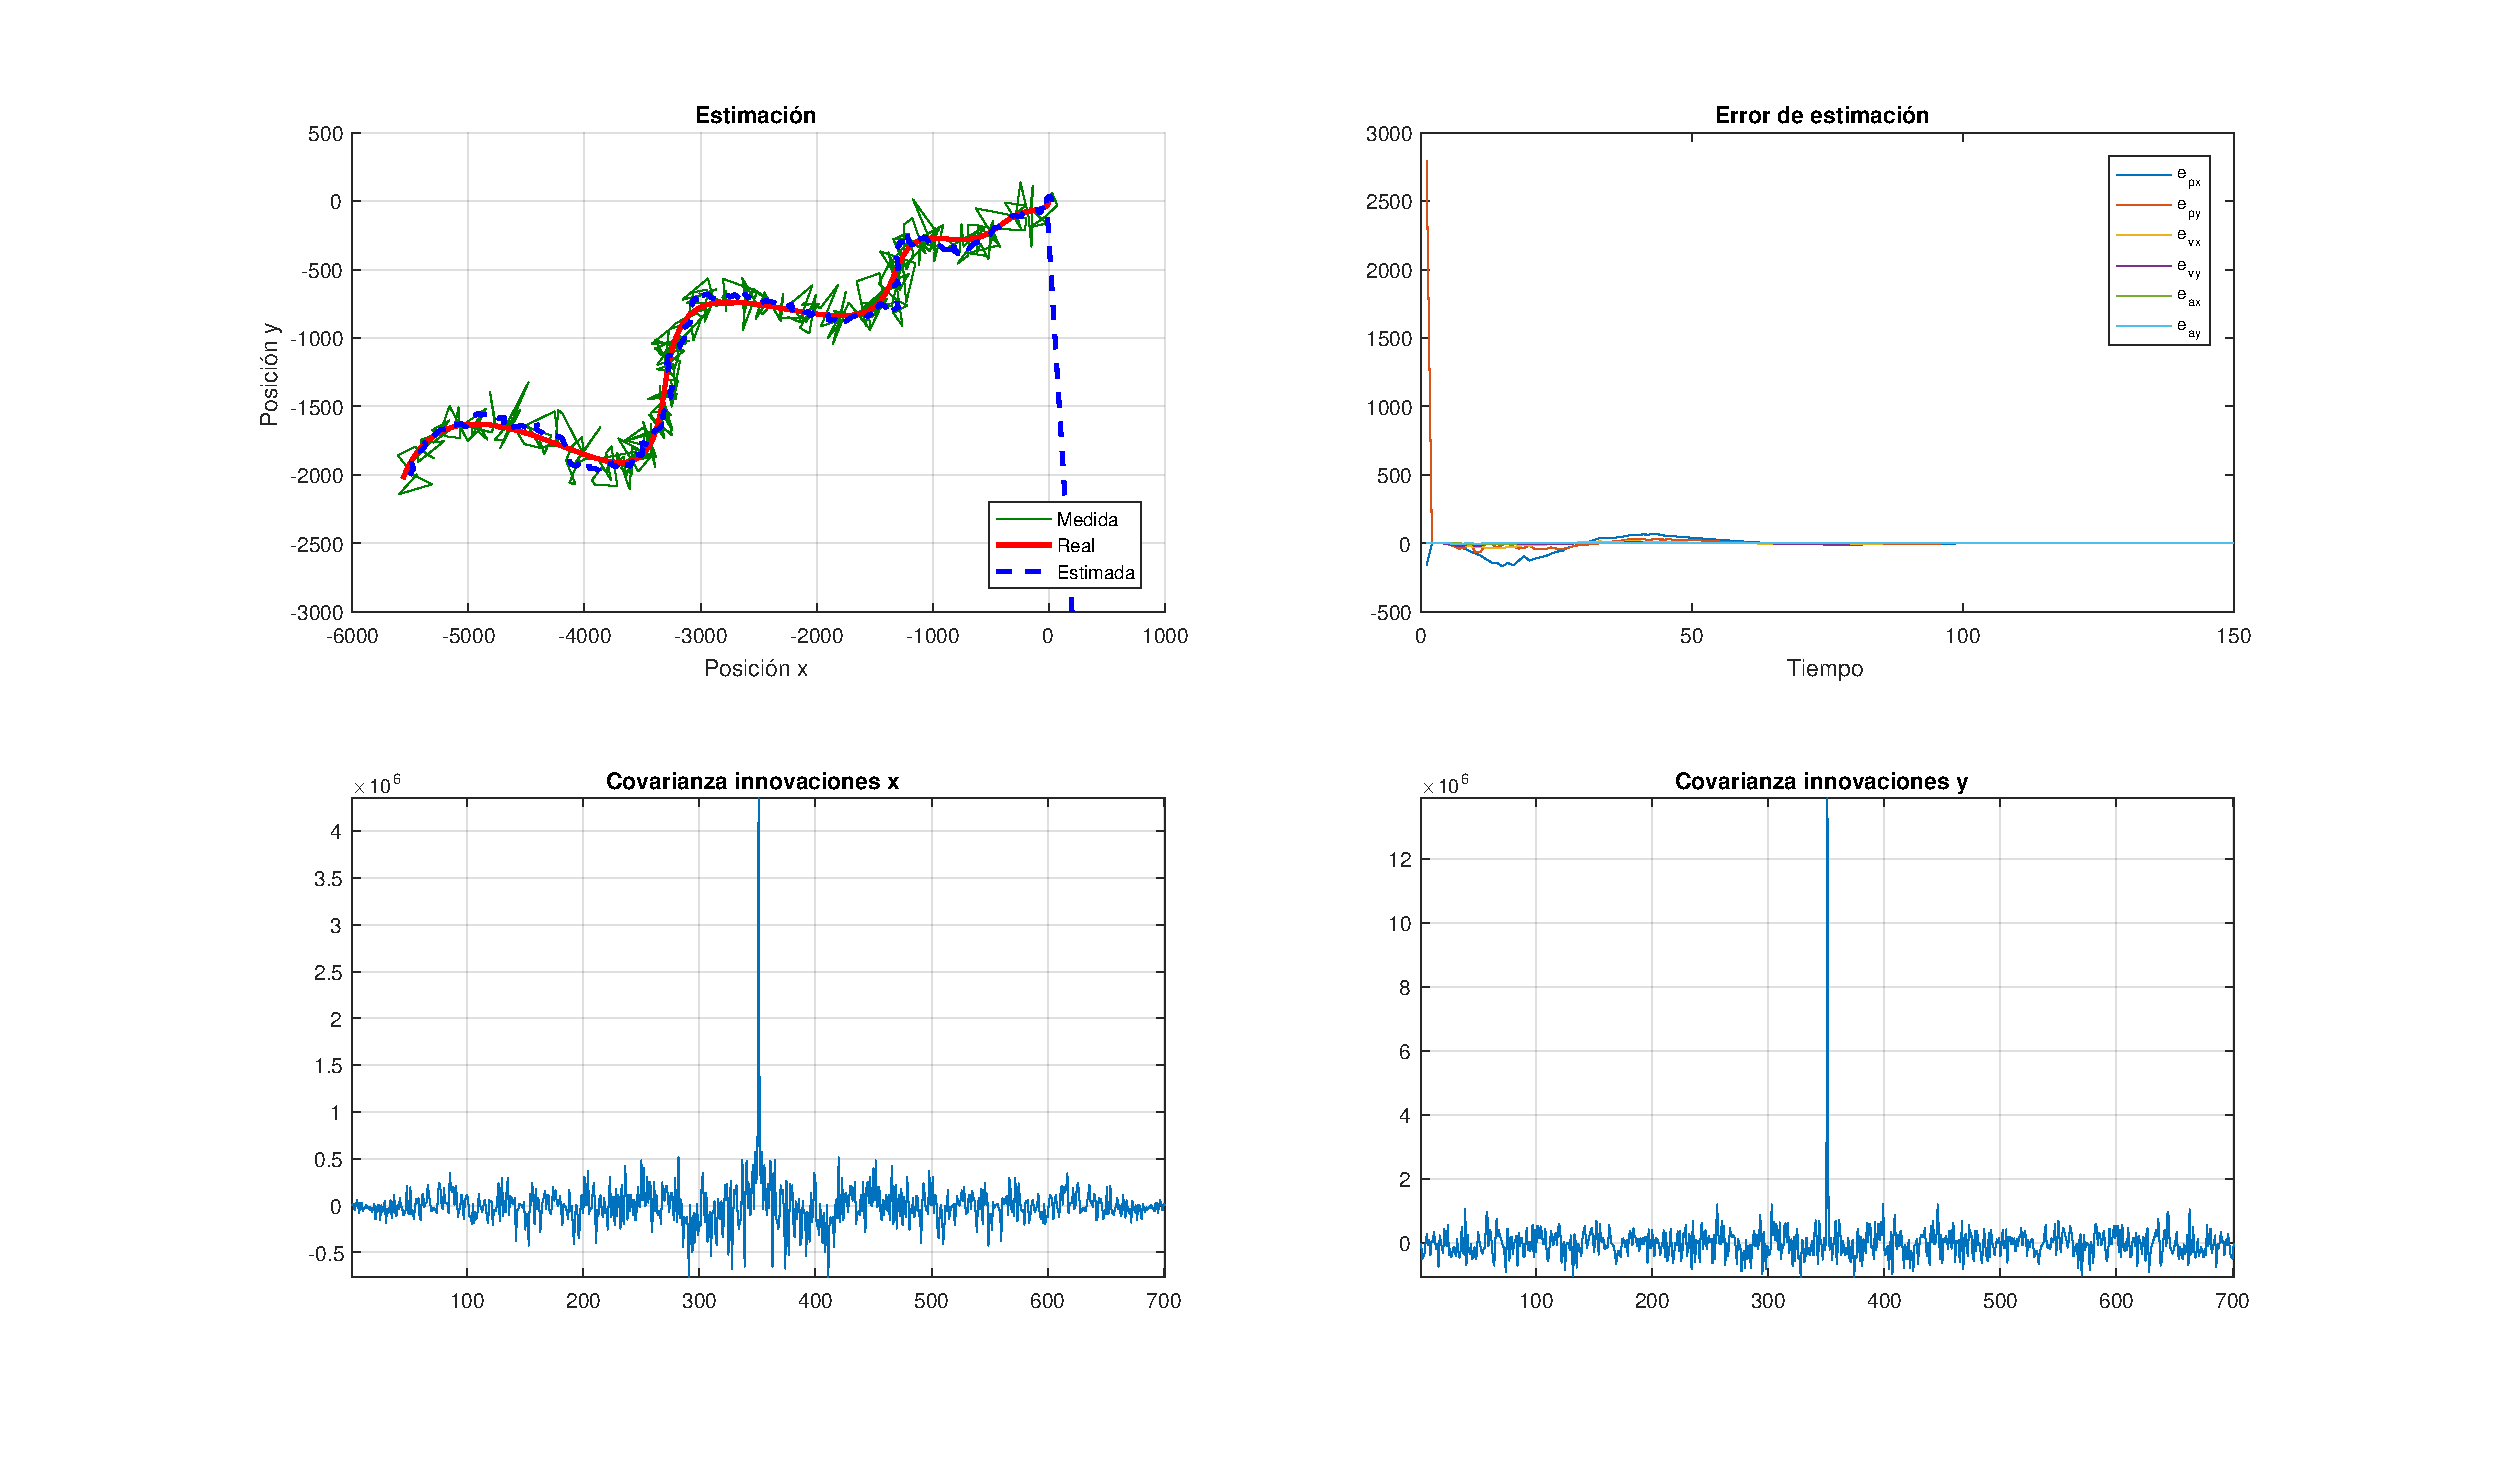
\includegraphics[scale=0.5,trim={6,5cm 0 0 0}]{Figuras/graf_ej3d.pdf}
			\caption{Caso 4}
			\label{fig:ej3d}
		\end{figure}
		
%	\subsection{Script}
%	
%		A continuación presentamos el script de esta sección. Básicamente realiza lo mismo que el punto anterior pero para distintas condiciones iniciales.
%
%	\lstinputlisting[]{EJ3.m}
	
